\section{Mode d'emploi}
1. Allumer l'Arduino. \color{red} Explain how to do that with a picture \color{black}\\

2. "Pairer" le smartphone avec l'Arduino
\begin{figure}[H]
	\begin{center}
		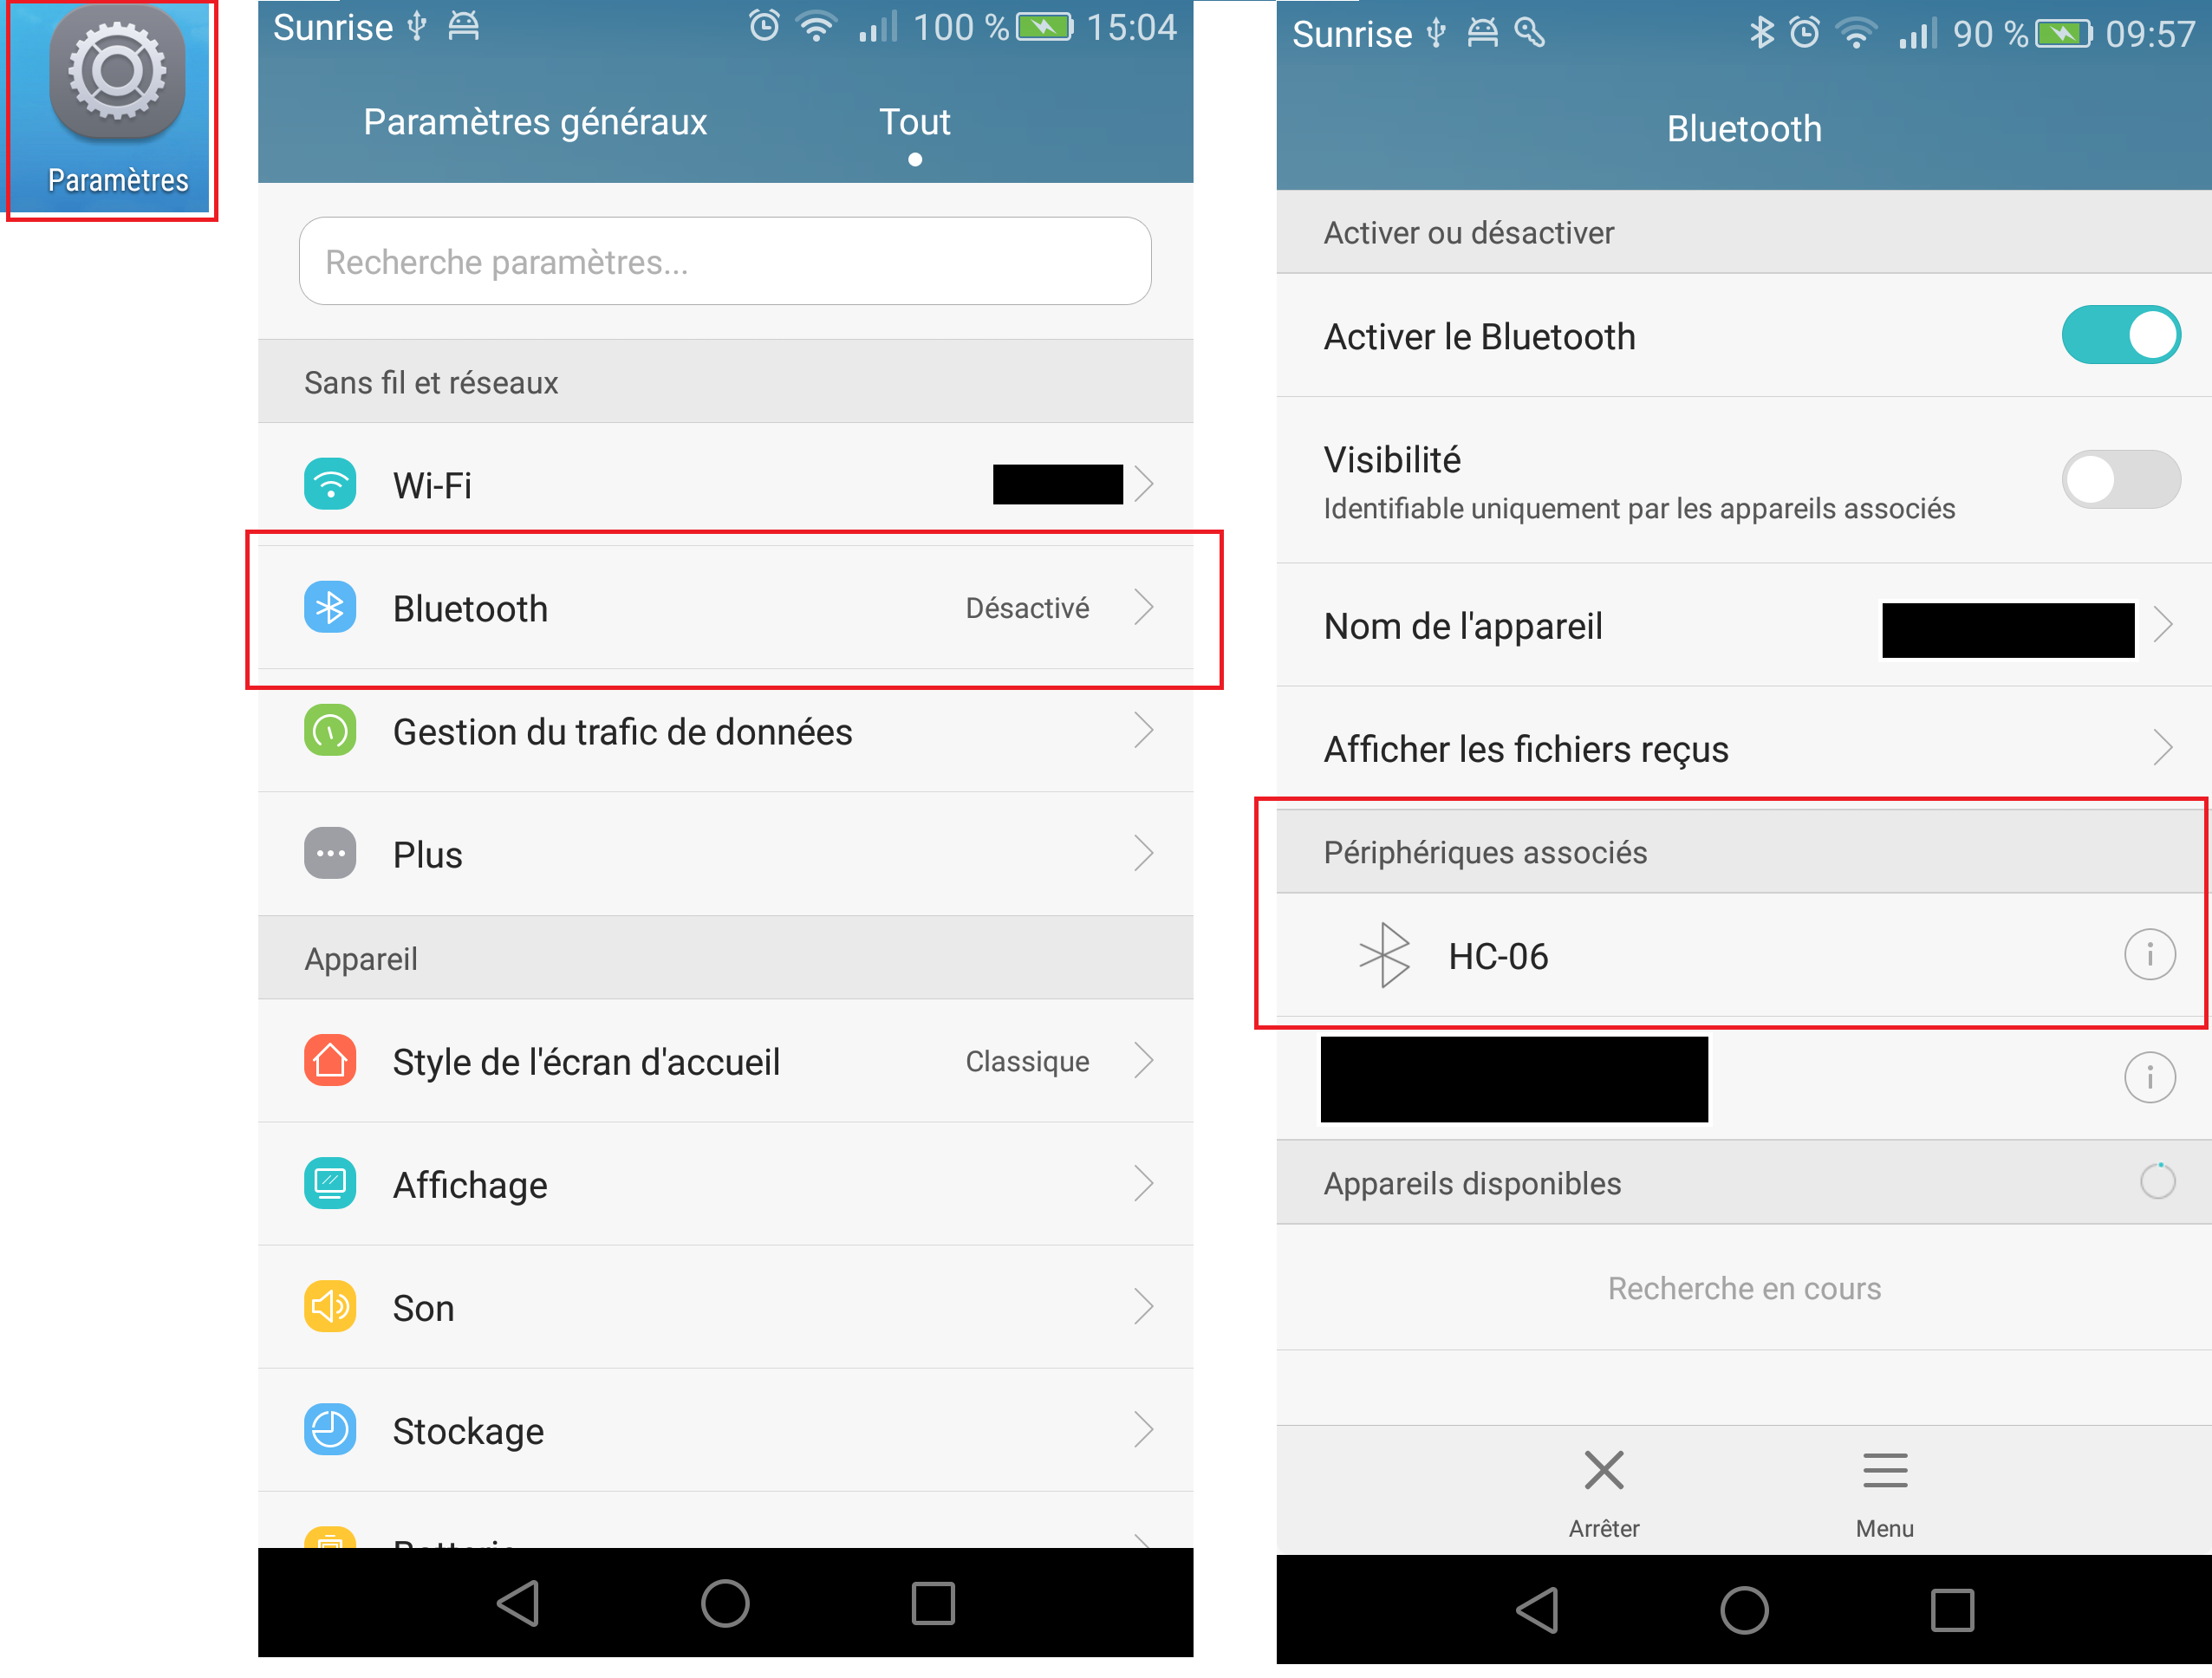
\includegraphics[width=15cm]{img/pairDevice.png}
		\caption{Pairage avec l'Arduino}
		\label{paired}
	\end{center}
\end{figure}
3. Une fois l'Arduino pairé, on peut lancer l'application Android
\begin{figure}[H]
	\begin{center}
		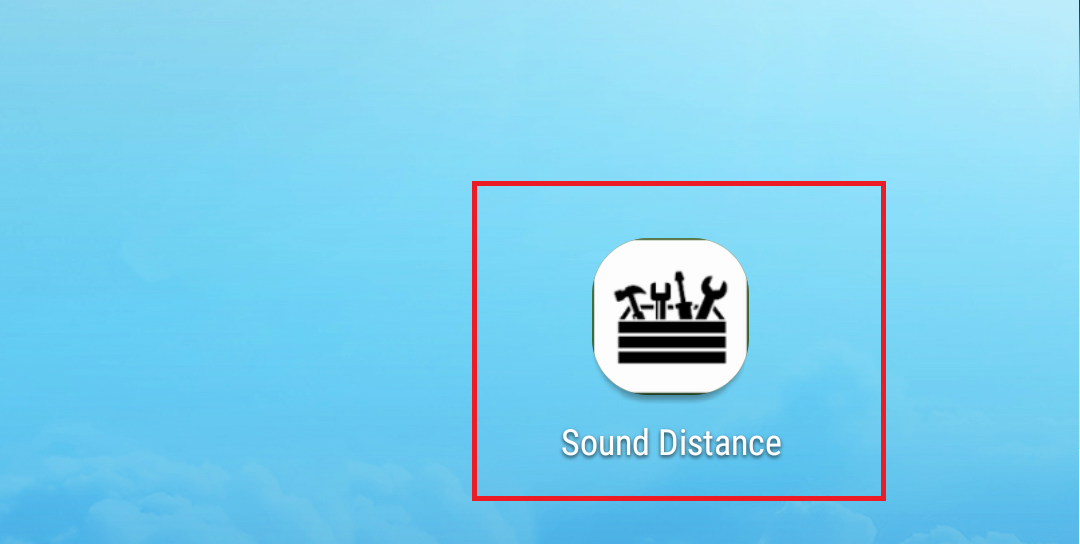
\includegraphics[width=10cm]{img/logo.png}
		\caption{Icône de lancement de l'application}
		\label{launch}
	\end{center}
\end{figure}
4. On arrive sur la liste des mesures précédemment réalisées. Toutes les mesures réalisées sont enregistrées dans un fichier externe et rechargées au lancement de l'application.\\ En cliquant sur un élément de la liste, on peut voir des informations supplémentaires. En faisant un long clic sur l'un des éléments de la liste, un menu d'actions s'affiche.
\begin{figure}[H]
	\begin{center}
		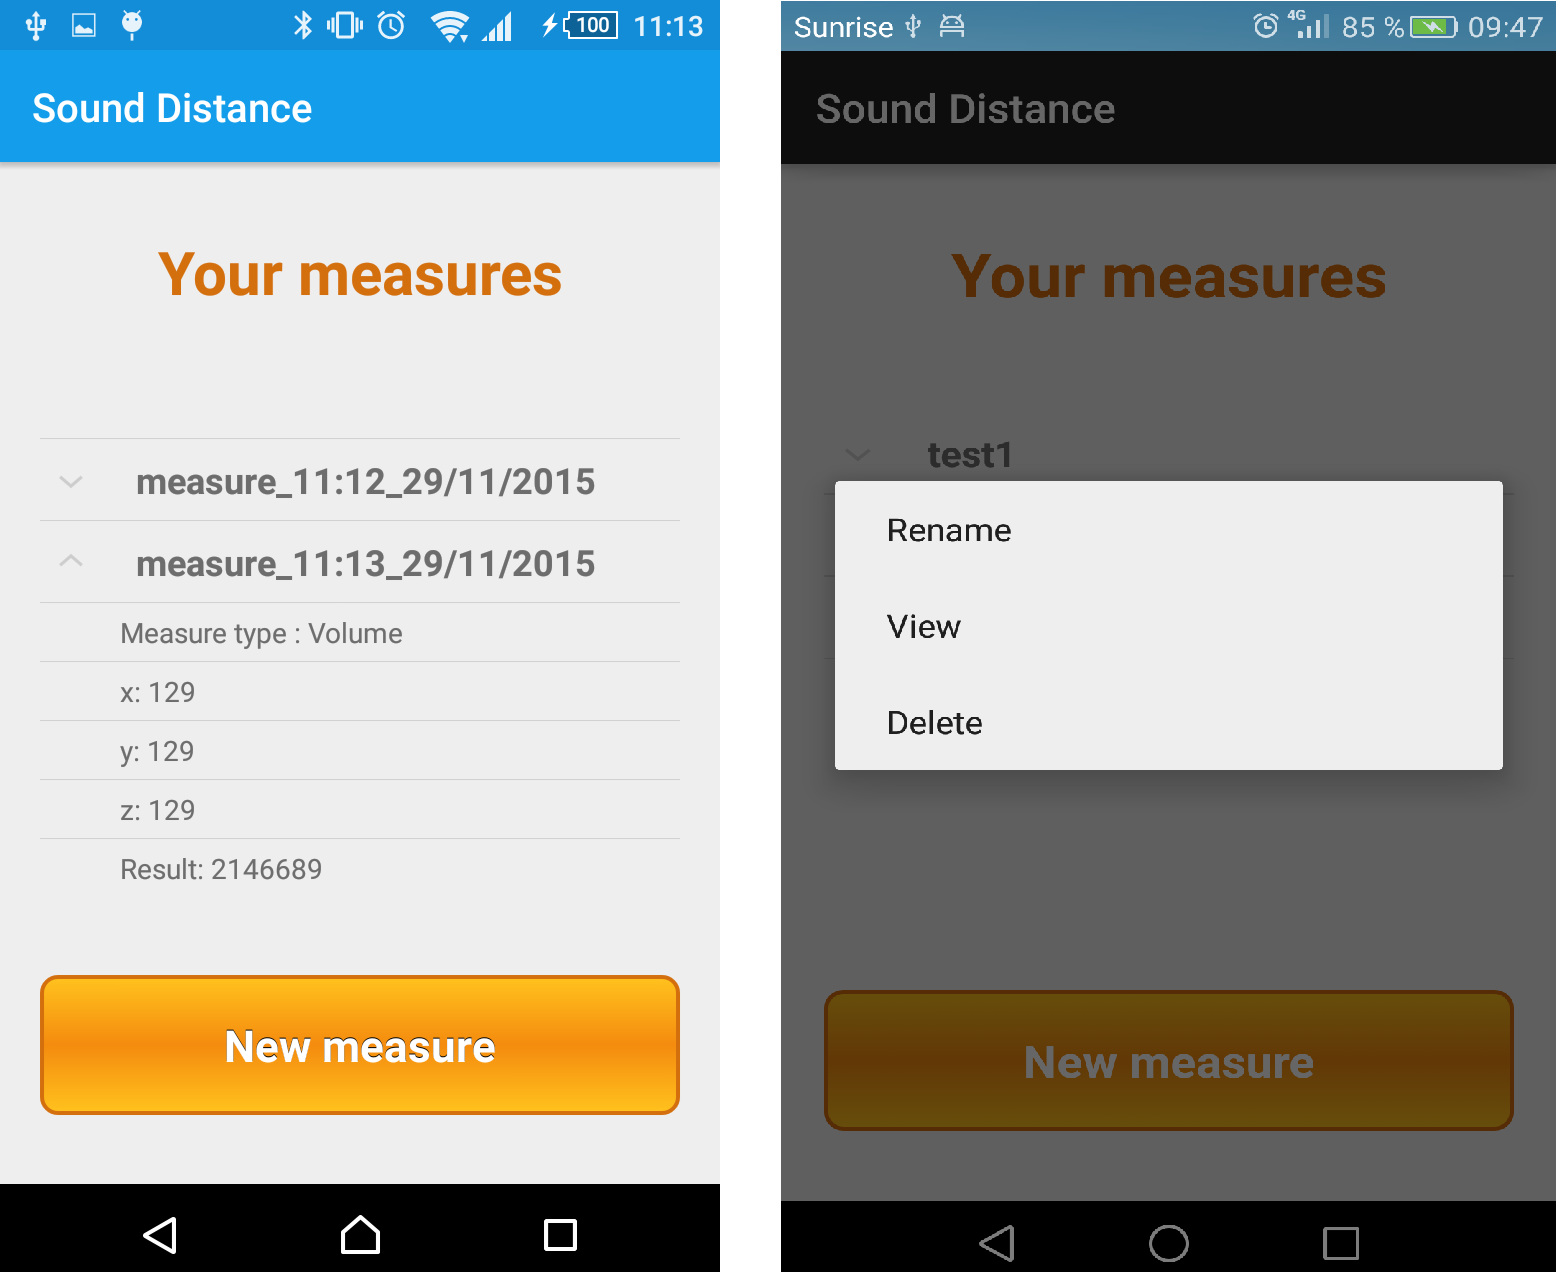
\includegraphics[width=12cm]{img/mesureList.png}
		\caption{Liste des mesures}
		\label{mesureList}
	\end{center}
\end{figure}
4.a) Gestion des mesures: Trois actions sont disponibles sur les mesures:
\begin{enumerate}
	\item Rename : Renomme la mesure
	\begin{figure}[H]
		\begin{center}
			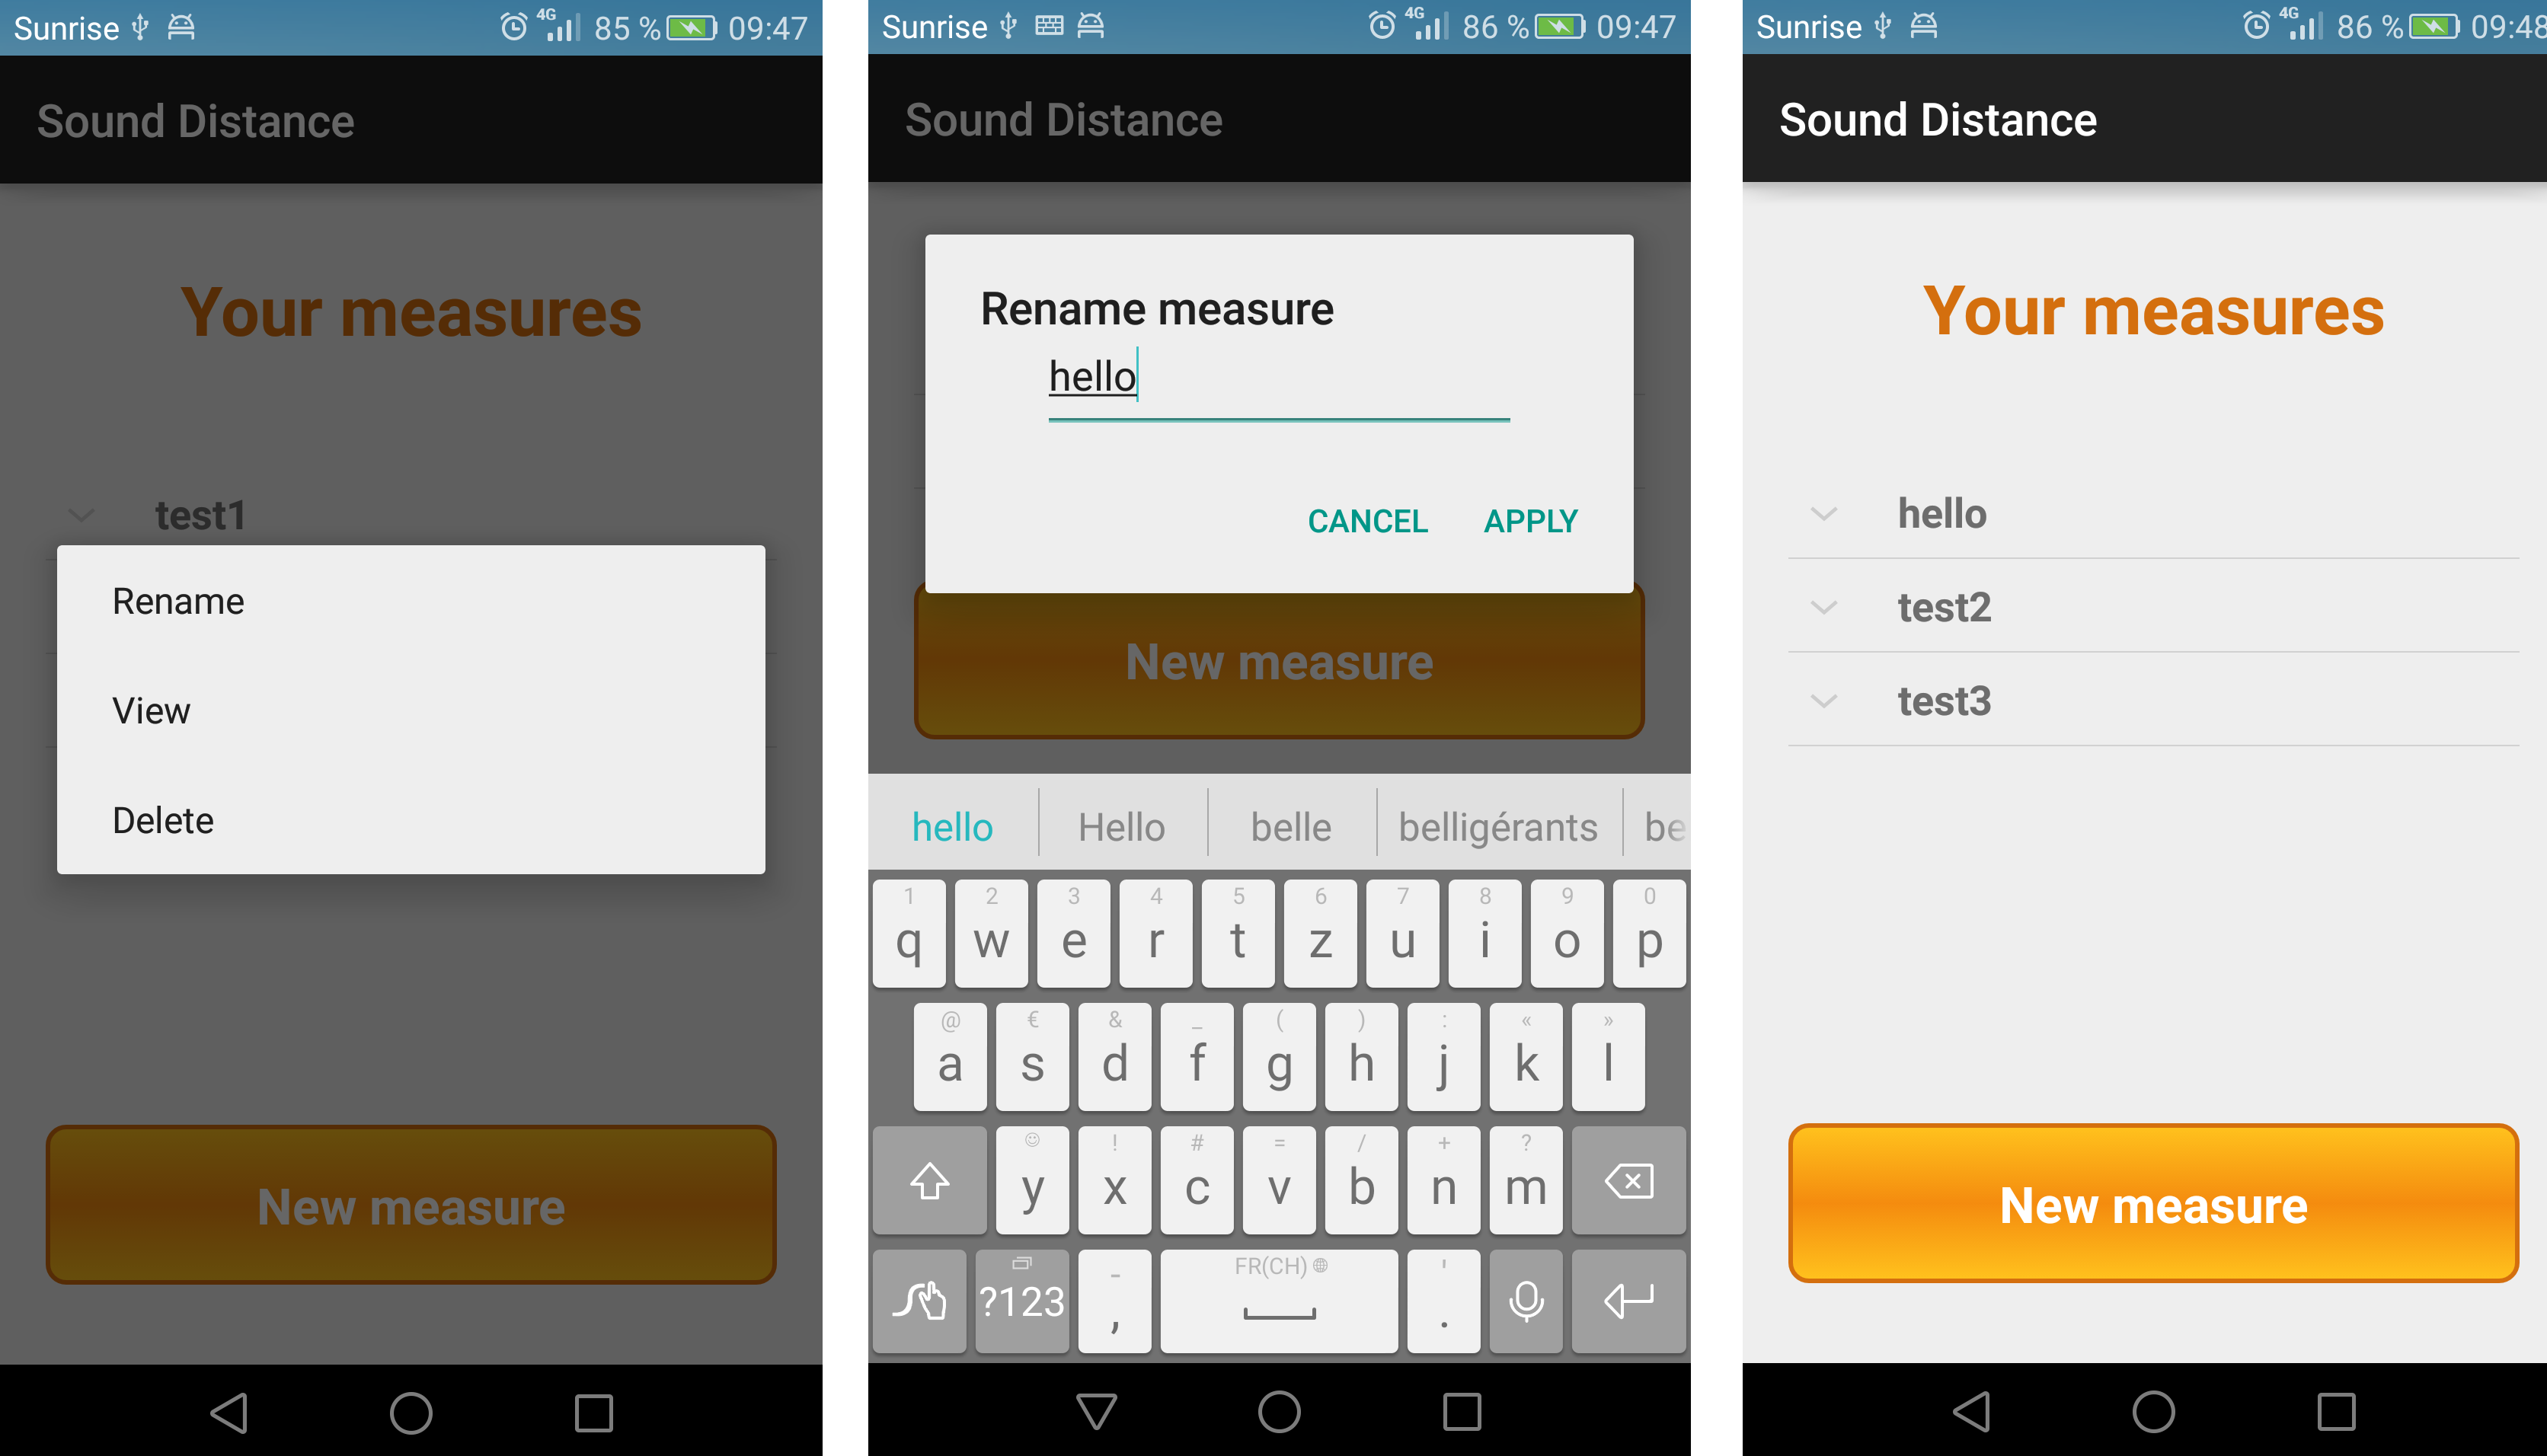
\includegraphics[width=16cm]{img/renameMeas.png}
			\caption{Modification du nom de la mesure}
			\label{rename}
		\end{center}
	\end{figure}
	\item Delete : Supprime la mesure de la liste
	\begin{figure}[H]
		\begin{center}
			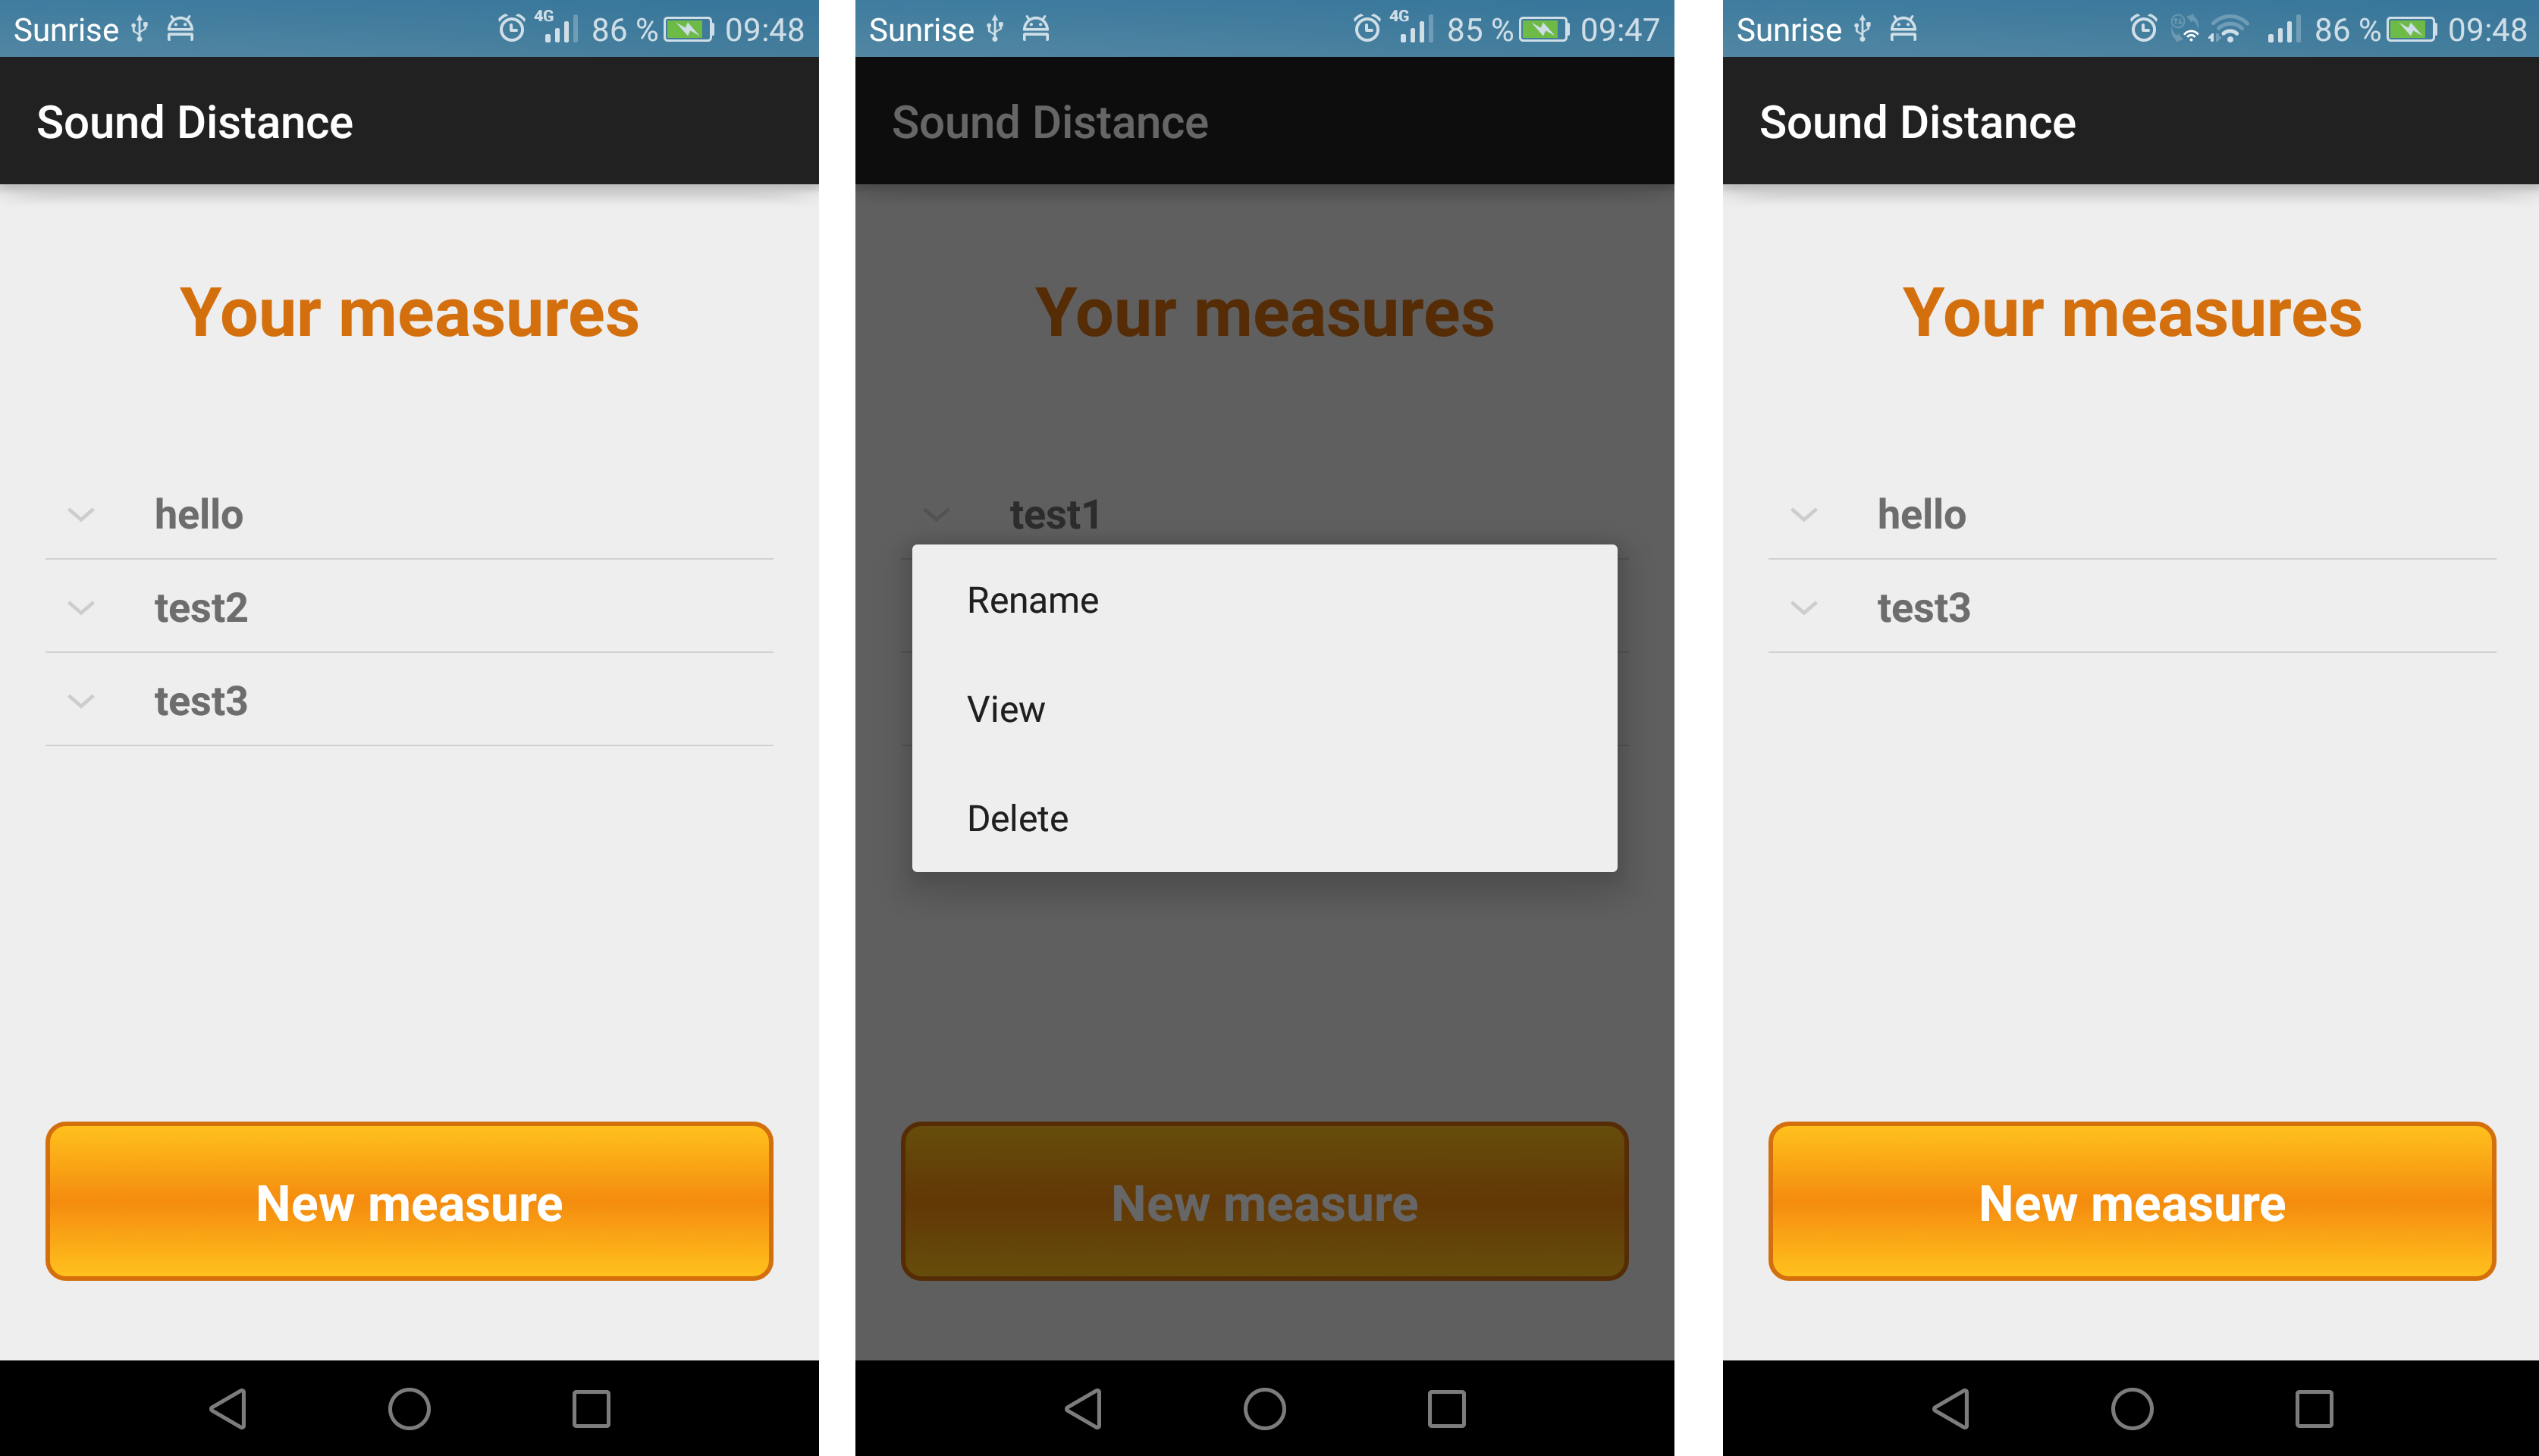
\includegraphics[width=16cm]{img/deleteMeas.png}
			\caption{Suppression d'une mesure}
			\label{delete}
		\end{center}
	\end{figure}
	\item View : Lance la vue de visualisation de mesures. En fonction du type de mesure, l'affichage est différent. Le bouton return permet de revenir à la liste.
	\begin{figure}[H]
		\begin{center}
			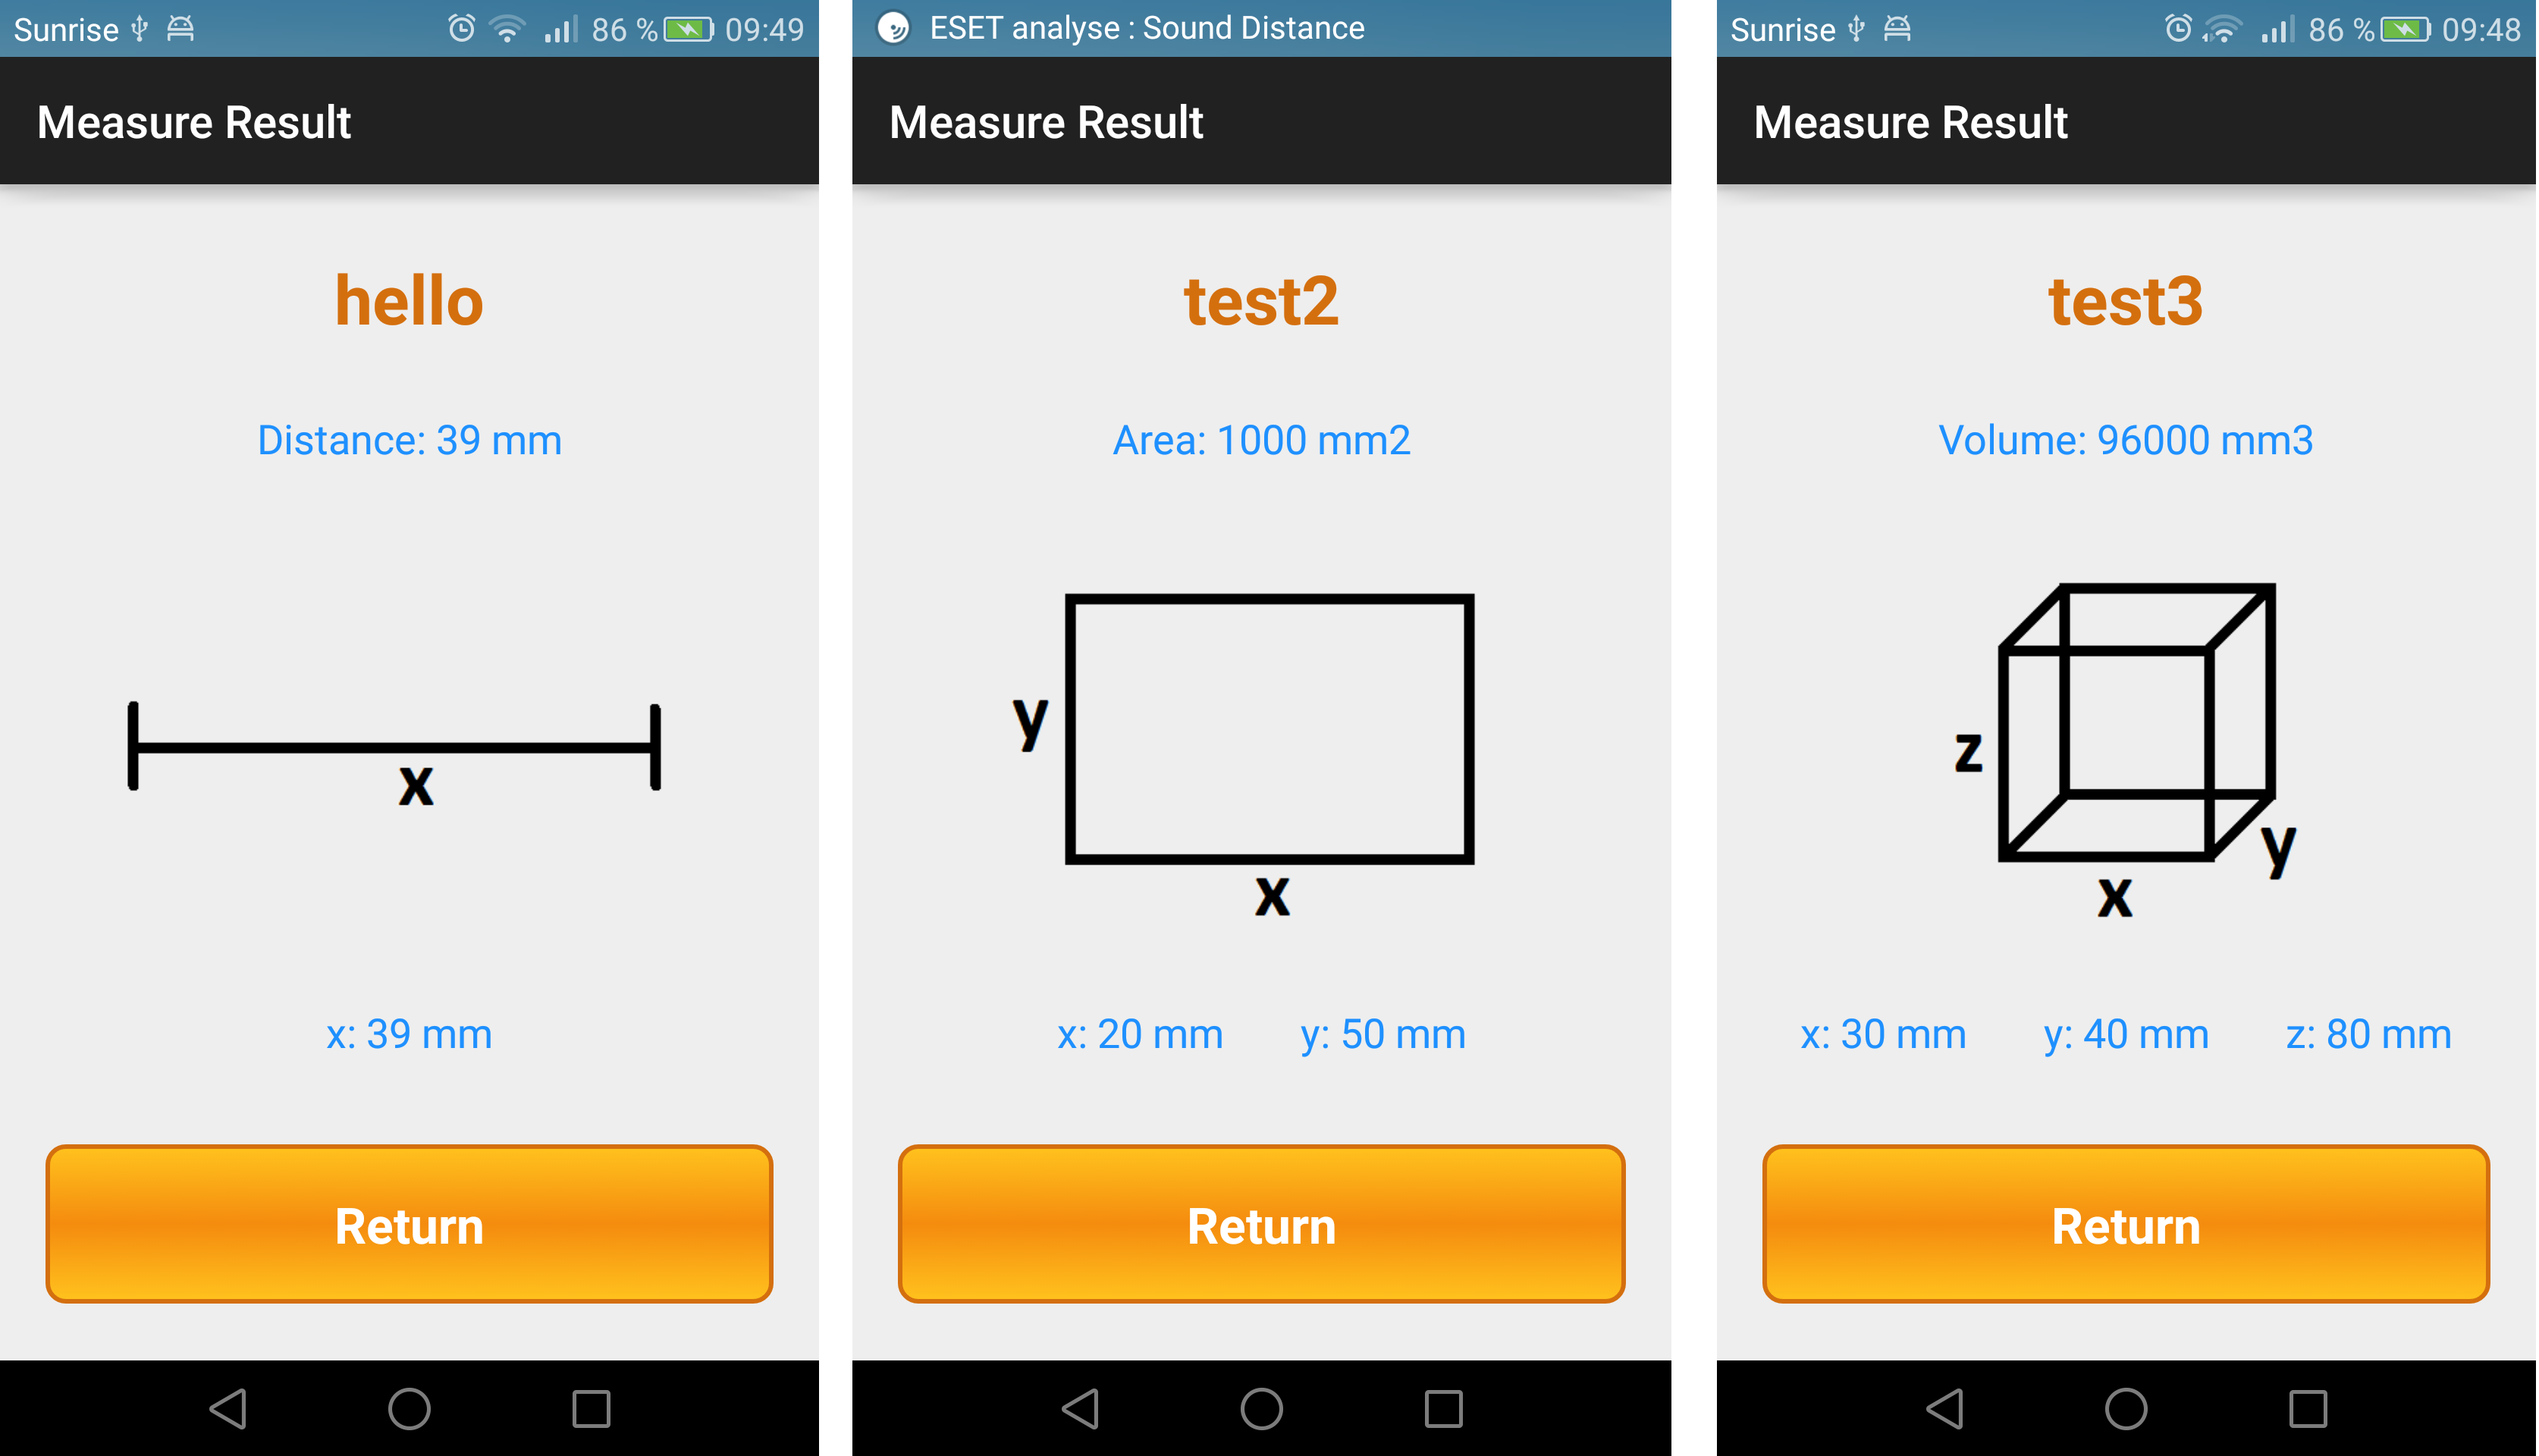
\includegraphics[width=16cm]{img/viewMeas.png}
			\caption{Visualisation d'une mesure - Distance, Area, Volume}
			\label{view}
		\end{center}
	\end{figure}
\end{enumerate}
4.b) Pour lancer une nouvelle mesure, il suffit de presser le bouton New measure. Cela va lancer l'écran de choix du type de mesure (Distance, area, volume). Une fois le type choisi, il faut presser le bouton Apply.
\begin{figure}[H]
	\begin{center}
		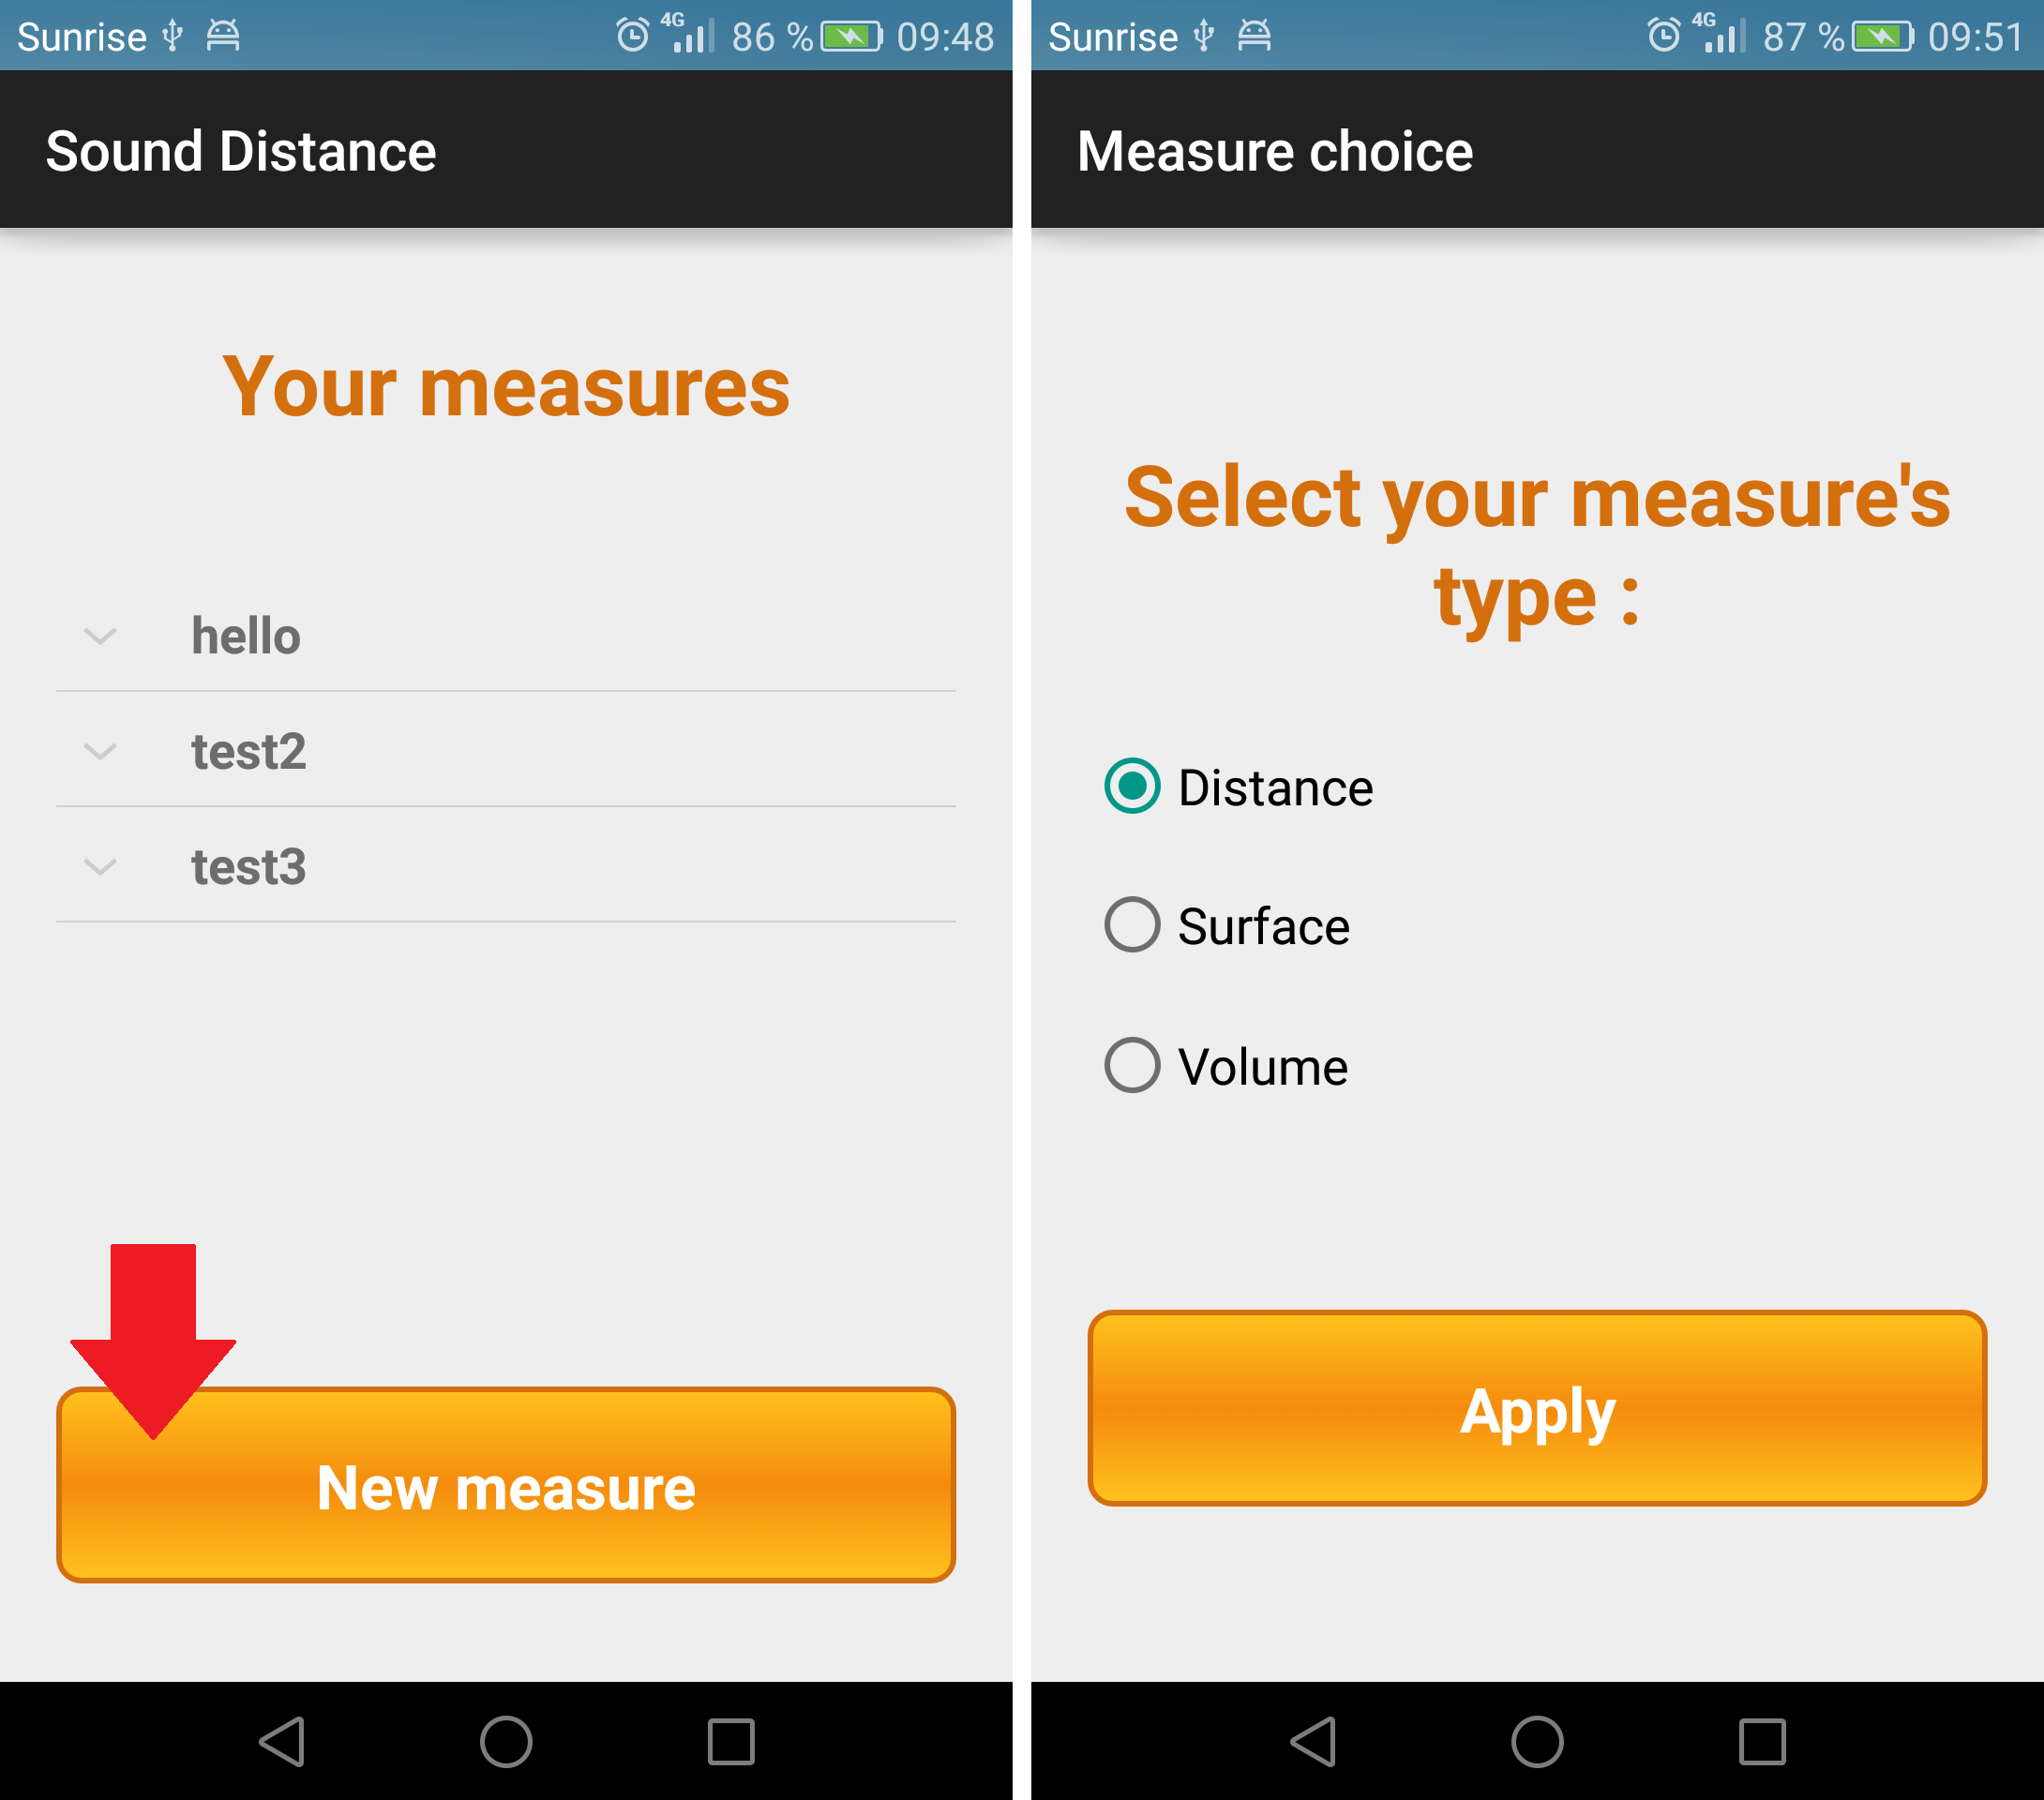
\includegraphics[width=9cm]{img/newMeas.png}
		\caption{Réalisation d'une nouvelle mesure}
		\label{newMeas}
	\end{center}
\end{figure}
5. On arrive ensuite sur l'écran de connexion Bluetooth. La liste des périphérique déjà pairés est affichée. Un clique sur un des éléments lance la connexion. Si la connexion échoue, un message toast nous en informe. Sinon, l'écran de mesure s'affiche.
\begin{figure}[H]
	\begin{center}
		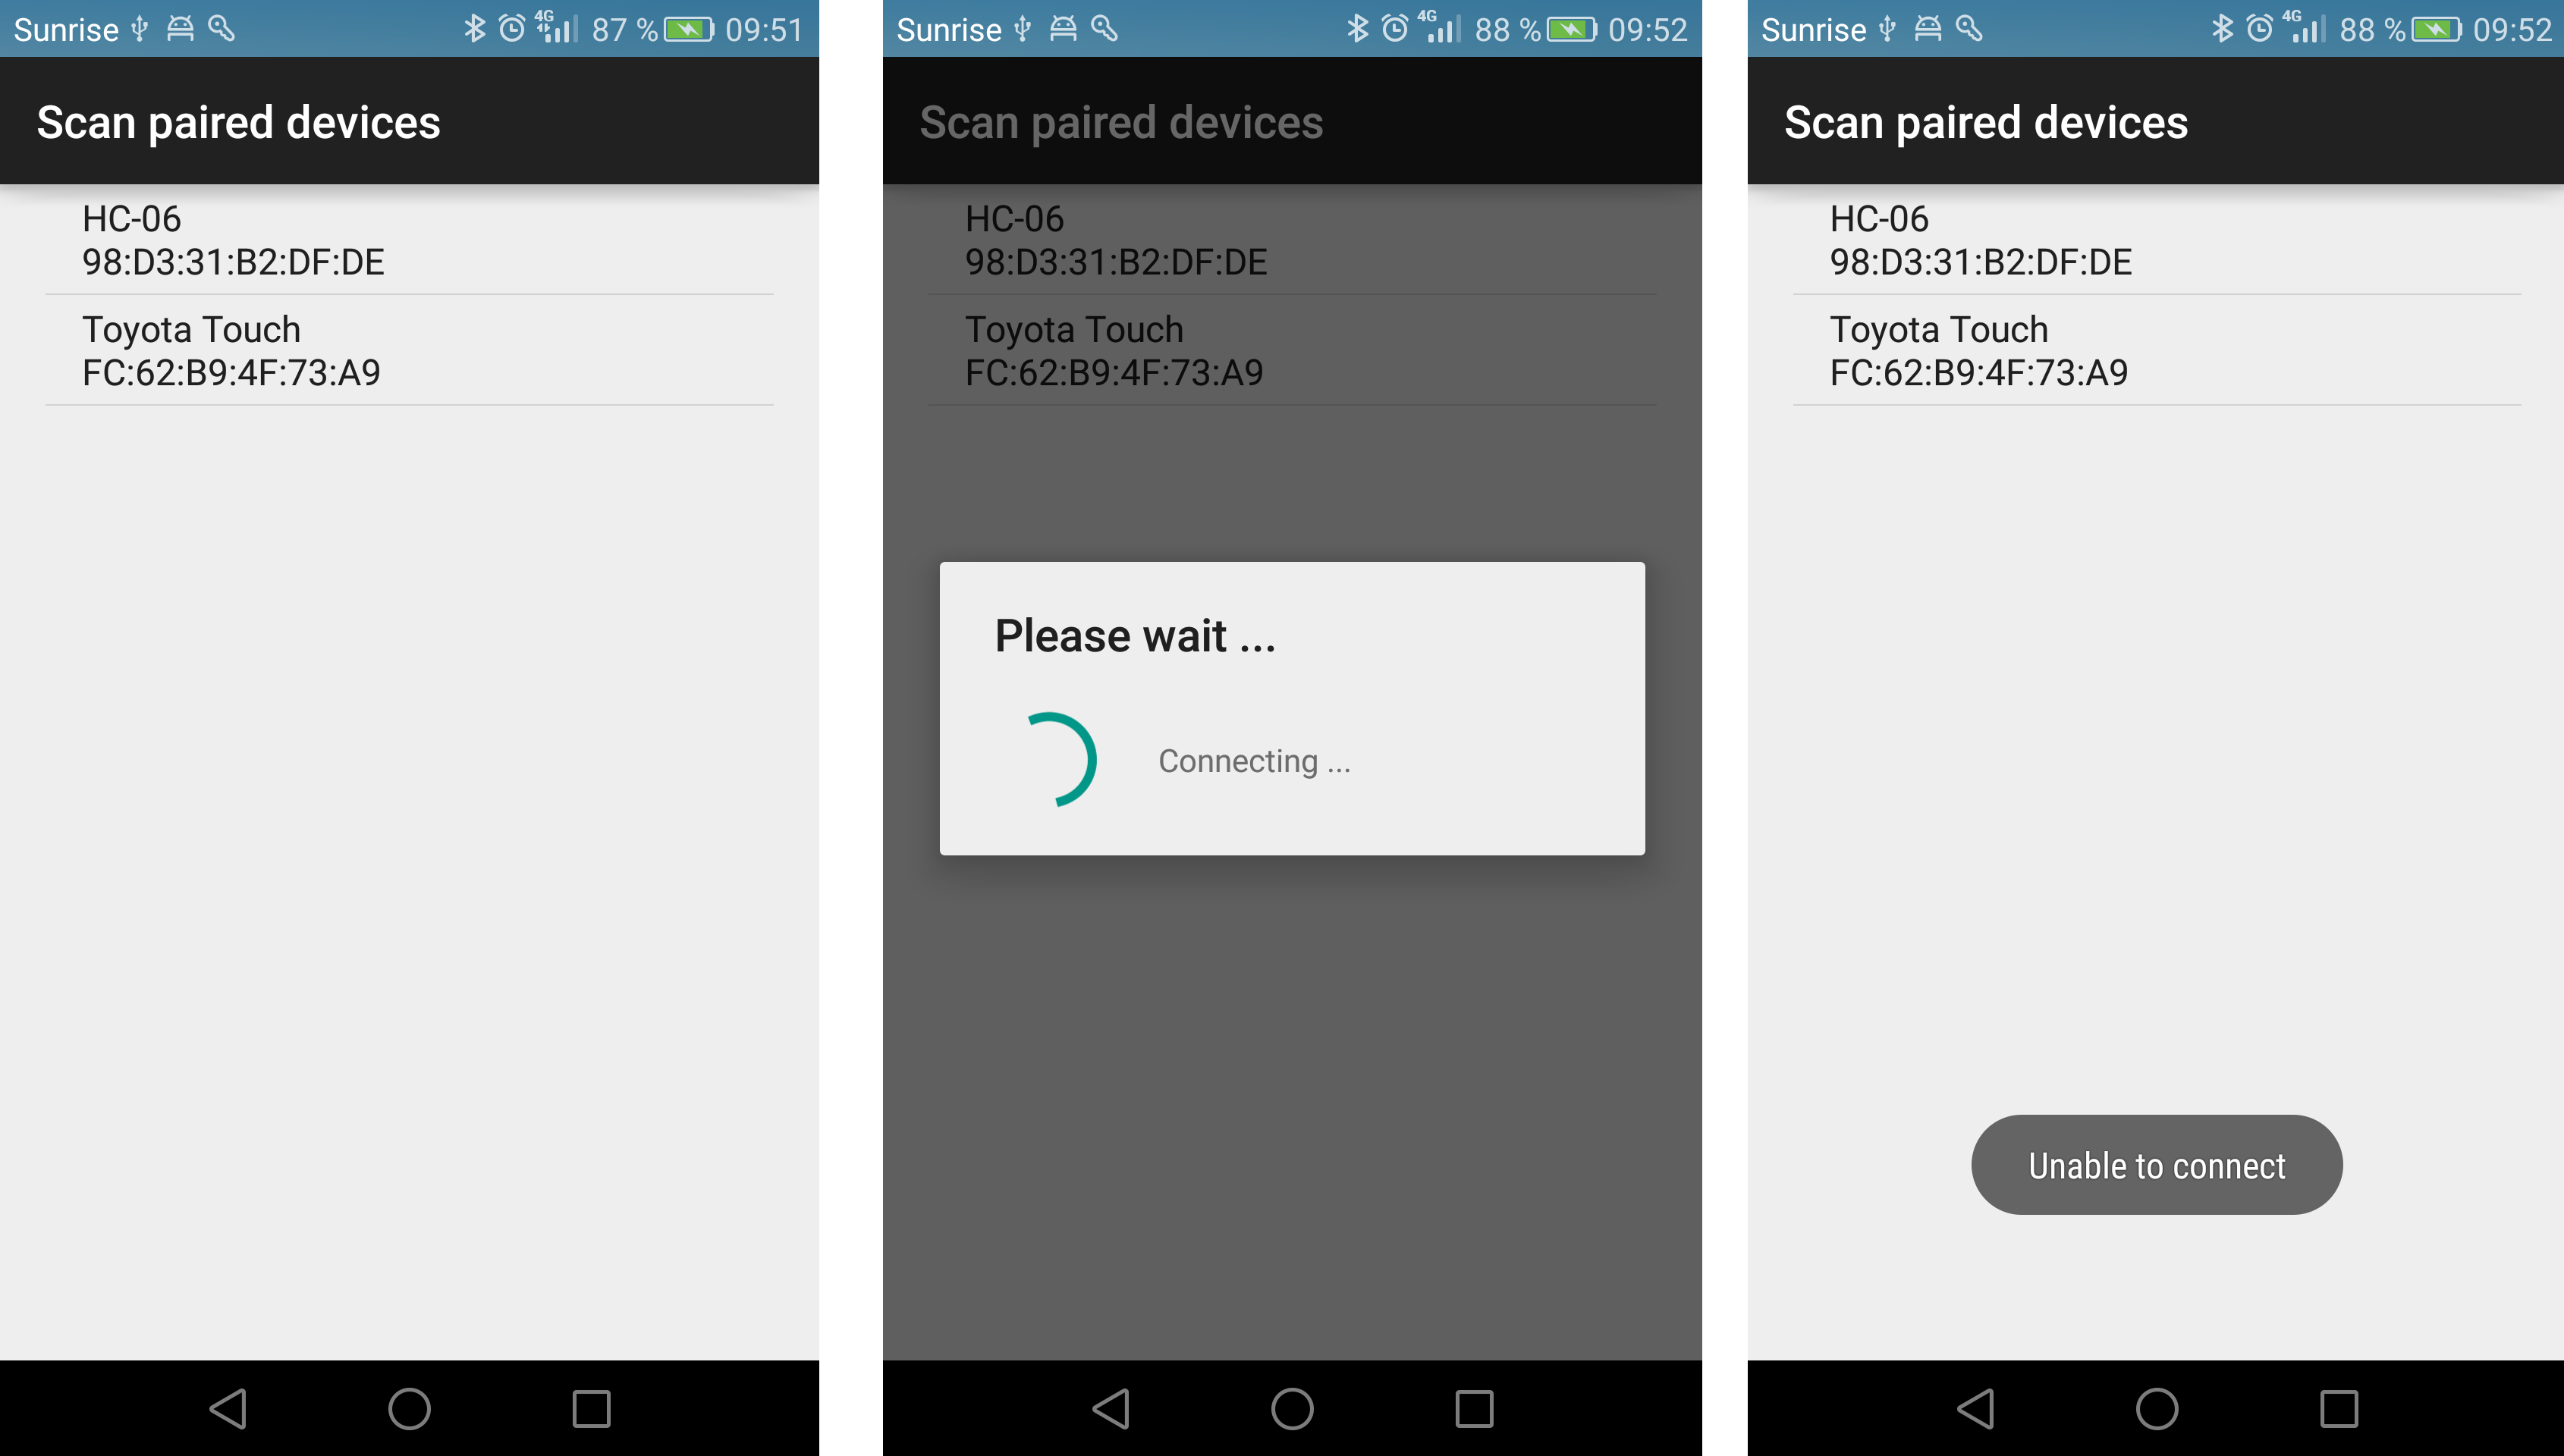
\includegraphics[width=14cm]{img/bluetooth.png}
		\caption{Connexion Bluetooth}
		\label{bluetooth}
	\end{center}
\end{figure}
\textbf{Information: } L'activation du Bluetooth est faite automatiquement par l'application sans demander la permission par souci de simplicité d'utilisation.\\
